\documentclass[12pt,a4paper]{article}

\usepackage[left=3cm, right=3cm, top=2.5cm, bottom=2.5cm]{geometry}
\usepackage{setspace}
\usepackage{amsmath}
\usepackage{tikz}
\usepackage{pgfplotstable}
\usepackage{titlesec}
\usepackage{bm}
\usepackage{tcolorbox}
\tcbuselibrary{skins}
\usepackage{empheq}
\usepackage{booktabs}
\usepackage{caption}
\usepackage{hyperref}
\usepackage{fancyhdr}
\hypersetup{
    colorlinks=true,
    linkcolor=black,
    filecolor=magenta,      
    urlcolor=cyan,
    pdfpagemode=FullScreen,
    }
\usepackage{graphicx}
\graphicspath{ {./images/} }


\titleformat{\section}{\Large\bfseries}{\thesection}{1em}{}
\titleformat{\subsection}{\large\bfseries}{\thesubsection}{1em}{}


\renewcommand{\contentsname}{Table des Matières}
%\renewcommand{\baselinestretch}{1.5}

\title{Étude des équations balistiques}
\author{Liviu Arsenescu, Cătălin Bozan}
\date{date}

\newtcbox{\mymath}[1][]{%
    nobeforeafter,
    math upper,
    tcbox raise base,
    enhanced,
    colframe=black,
    colback=white,
    boxrule=1pt,
    drop shadow={
        shadow xshift=3pt,
        shadow yshift=-3pt,
        opacity=1
    },
    #1
}

\pagestyle{fancy}
\fancyhf{}
\rhead{\includegraphics[width=4cm]{hearclogo.png}}
\lhead{\thepage}
\setlength{\headsep}{30pt}

\begin{document}
    \pagenumbering{gobble}
    \begin{titlepage}
        \begin{center}
            \vspace*{\fill}
            \Huge \textbf{Étude des équations de la balistique :} \\
            \Huge \textbf{Équations du mouvement dans un champ gravitationnel} \\
            \Large Rapport du Laboratoire \\
            \begin{figure}[h]
                \centering
                \includegraphics[width=7cm]{hearclogo.png}
            \end{figure}
            \vspace{\fill}
            \Large Liviu Arsenescu, Cătălin Bozan \\
            19.03.2024

            \vspace*{\fill}
        \end{center}
    \end{titlepage}

    \thispagestyle{empty}
    \tableofcontents
    \newpage

    \pagenumbering{arabic}
    \section{Description de l'expérience}
    \subsection{Buts}
    \begin{itemize}
        \item Vérifier les équations de la balistique
        \item Obtenit la vitesse à laquelle le canon tire le boulet
        \item Pédire la hauteur de l'impact de la bille contre un mur avec un tir oblique
    \end{itemize}

    \subsection{Éléments théoriques}
    \subsubsection{Les différentes grandeurs physiques rencontrées}
    \begin{minipage}{0.6\linewidth}
        \begin{itemize}
            \item \textbf{h} - hauteur initiale 
            \item \textbf{d} - distance entre le canon et le point d'impact 
            \item \textbf{H} - hauteur d'impact
            \item $\bm{\theta}$ - angle de tir 
            \item $\bm{v_0}$ - vitesse de sortie du canon
        \end{itemize}
    \end{minipage}%
    \hfill
    \begin{minipage}{0.4\linewidth}
        \begin{itemize}
            \item[-] $\bm{[h]=cm}$
            \item[-] $\bm{[d]=cm}$
            \item[-] $\bm{[H]=cm}$
            \item[-] $\bm{[\theta]=deg}$
            \item[-] $\bm{[v_0]=cms^{-1}}$
        \end{itemize}   
    \end{minipage}
    \subsubsection{Les équations de la balistique}
    Dans le cas du mouvement qui nous intéresse, on peut observer deux types de mouvements :
    \begin{enumerate}
        \item Mouvement à vitesse constante, avec l'équation :
        \begin{align*}
            x(t) = v_xt + x_0
        \end{align*}
        \item Mouvement à accélération constante, avec les équations :
        \begin{align*}
            v_x(t) &= a_xt + v_{x0} \\
            x(t) &= \frac{1}{2}a_xt^2 + v_x(t) + x_0
        \end{align*}
    \end{enumerate}
    Où $x(t)$ est le déplacement sur n'importe quel axe de nom x, en fonction du temps, $v_x(t)$ est la vitesse sur l'axe x et $a_x$ est l'accélération. \\
    Pour étudier le tir au canon, on a les contraintes mathématiques suivantes :
    \begin{equation*}
        \vec{v_0}=
        \begin{pmatrix}
            v_{x0} \\
            v_{y0}
        \end{pmatrix}, 
        \|\vec{v_0}\|=v_0
    \end{equation*}
    \begin{itemize}
        \item Pour l'axe x :
        \begin{align*}
            x_0 &= 0 \\
            v_x(t)&=v_0cos(\theta_0)
        \end{align*}
        \item Pour l'axe y :
        \begin{align*}
            a_y &= -g \\
            v_{y0} &= v_0sin(\theta_0) \\
            y_0 &= h
        \end{align*}
        Où :
        \begin{itemize}
            \item $v_0$ - vitesse de sortie du canon
            \item $\theta_0$ - angle entre $\vec{v_0}$ et l'axe x
            \item $g$ - accélération gravitationnelle de Terre
            \item $h$ - hauteur de départ
        \end{itemize}
    \end{itemize}
    Avec ces contraintes, on peut construire le système d'équations suivant pour le mouvement que on étudie :
    \begin{center}
        \vspace{-\baselineskip}
        \begin{minipage}{0.3\linewidth}
            \begin{empheq}[box={\mymath}]{align*}
                x(t) &= v_0cos(\theta_0)t \\
                v_x(t) &= v_0cos(\theta_0)
            \end{align*}
        \end{minipage}%
        \begin{minipage}{0.1\linewidth}
            \begin{center}
                et
            \end{center}
        \end{minipage}%
        \begin{minipage}{0.4\linewidth}
            \begin{empheq}[box={\mymath}]{align*}
                y(t) &= \frac{-1}{2}gt^2 + v_0sin(\theta_0)t + h \\
                v_y(t) &= -gv_0sin(\theta_0) + v_0sin(\theta_0)
            \end{align*}
        \end{minipage}
    \end{center}
    \subsubsection{Tir horizontal :}
    Pour le tir horizontal, le vecteur vitesse fait avec l'axe x un angle $\theta$ de 0 degrées :
    \begin{align*}
        \vec{v_0}=
        \begin{pmatrix}
            v_{x0} \\
            v_{y0}
        \end{pmatrix}
        =
        \begin{pmatrix}
            v_{x0} \\
            0
        \end{pmatrix}
        &\Rightarrow \|\vec{v_0}\|=v_{x0}=v_0, \\
        cos(\theta)=1&, sin(\theta)=0
    \end{align*}
    Pour la position initiale($\vec{r_0}$), on a les valeurs suivantes :
    \begin{equation*}
        \vec{r_0}=
        \begin{pmatrix}
            x_0 \\
            y_0
        \end{pmatrix}
        =
        \begin{pmatrix}
            0 \\
            h
        \end{pmatrix}
    \end{equation*}
    Nos équations deviennent :
    \begin{itemize}
        \item Pour l'axe x :
        \begin{empheq}[box={\mymath}]{align*}
            x(t)&=v_0t \\
            v_x(t)&=v_0
        \end{align*}
        \item Pour l'axe y
        \begin{empheq}[box={\mymath}]{align*}
            y&=-\frac{1}{2}gt^2+h \\
            v_y(t)&=-gt
        \end{align*}
    \end{itemize}
    L'instant où l'objet touche le sol nous donne la distance horizontale entre le point de départ et le point d'arrivée (d) :
    \begin{align*}
        y(t_f)=0 &\Rightarrow t_f=\sqrt{\frac{2h}{g}} \\
        d = x(t_f) = &v_0\cdot t_f = v_0 \cdot \sqrt{\frac{2h}{g}}
    \end{align*}
    \subsection{Principe de l'expérience}
    
    
    \subsection{Schéma et montage de l’expérience}
    Pour réaliser l'expérience, nous avons besoin d'un dispositif qui lance une bille, d'un moyen de marquer avec précision l'endroit où la bille a atterri et d'un moyen pour changer la hauteur et l'angle du canon.
    Dans notre cas, nous avons utilisé :
    \begin{itemize}
        \item Un canon à ressort à angle variable
        \item Une bille en plastique
        \item Du papier
        \item Du papier carbone
        \item Des boîtes, sur lesquelles nous avons posé le canon pour changer la hauteur du canon.
    \end{itemize}  
    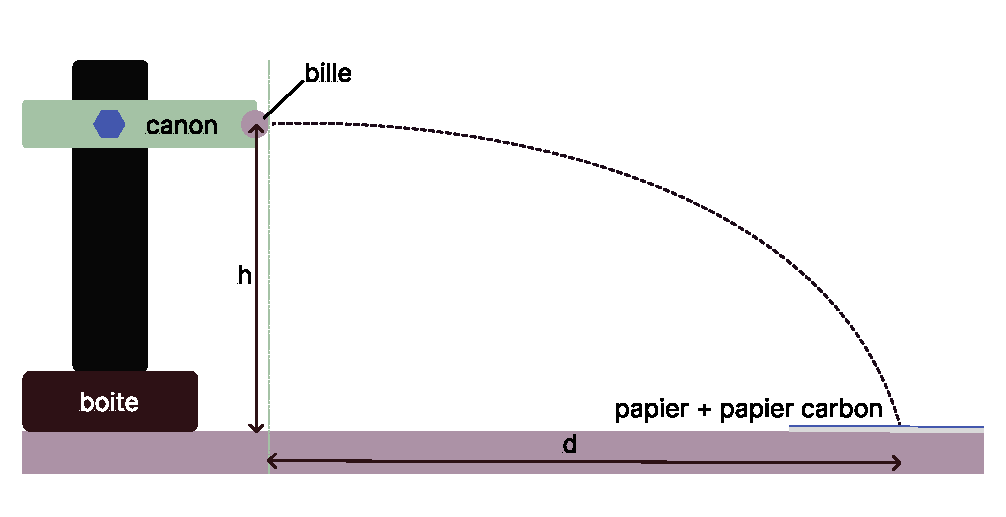
\includegraphics[width=0.4\paperwidth]{images/exp1_2.pdf}
    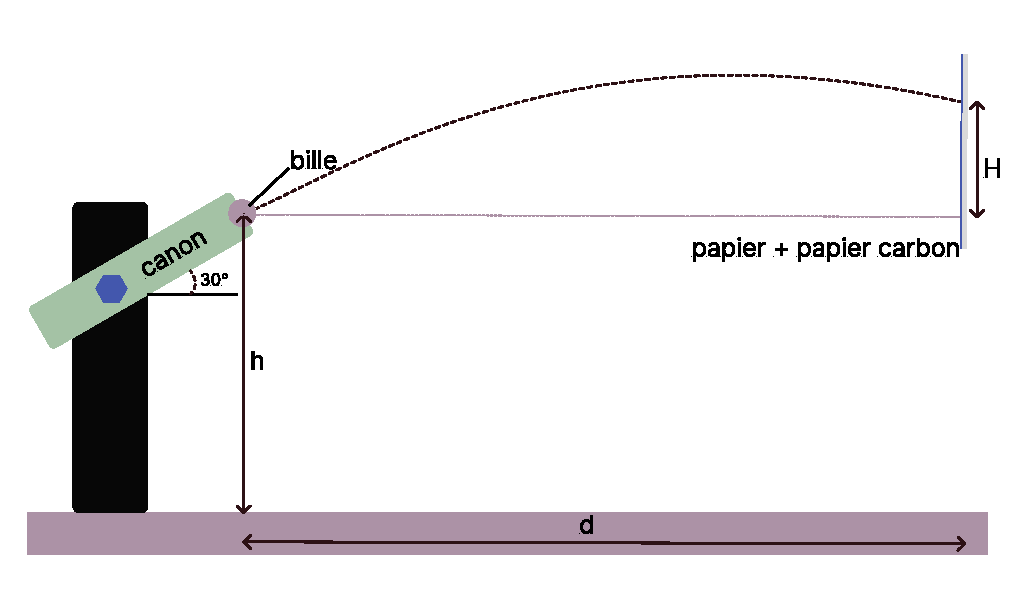
\includegraphics[width=0.4\paperwidth]{images/exp2_1.pdf}
    
    \subsection{Déroulement de l'expérience}
    \subsubsection{Tir horizontal : déduction la vitesse $v_0$ de sortie de la bille}
    \begin{itemize}
        \item Assurez-vous que le canon est réglé à un angle de zéro dégréé.
        \item Posez le canon sur le sol et tirez la bille en utilisant la puissance la plus faible du canon à ressort.
        \item Observez l'endroit où la bille a atterri et collez une feuille de papier sur le sol à l'endroit où la bille a atterri.
        \item Placez une feuille de papier carbone sur la feuille de papier.
        \item Tirez la bille cinq fois avec la même force de ressort afin de la faire tomber sur le papier carbone et de marquer sa position d'atterrissage.
        \item Mesurez la hauteur entre le sol et le bas de la marque de la bille sur le canon.
        \item Tracez des lignes perpendiculaires au canon qui passent par les marques laissées par la bille sur le papier carbone.
        \item Mesurer la distance entre les lignes perpendiculaires et la projection du centre de masse de la bille sur le sol.
        \item Utiliser des boîtes placées sous le canon pour modifier sa hauteur et répéter l'expérience pour \textbf{1000} hauteurs différentes.
        \item \textbf{We calculated stuff blabla}
    \end{itemize}

    \subsubsection{Tir oblique : Déduction de $H$ la hauteur de la bille par rapport à sa hauteur initiale $h$ après son lancement à $x = 70cm$ en utilisant la vitesse $v_0$ trouvée précédemment, et en comparant avec les mesures réelles.}

    \begin{itemize}
        \item Placer le canon à un angle de 30 degrés.
        \item Placez le canon de manière à ce qu'il y ait une distance de 70 cm entre le mur et le point où la bille toucherait le mur.
        \item Tirez une bille avec la puissance la plus faible du canon et collez une feuille de papier sur le mur à l'endroit où la bille a atterri.
        \item Coller le papier carbone sur la feuille de papier.
        \item Tirez la bille 5 fois avec le même réglage du canon, à la puissance la plus faible.
        \item Mesurez la distance entre les marques laissées par la bille sur le papier et le sol pour pouvoir déduire $H$, la différence de hauteur finale de la bille par rapport à sa hauteur initiale $h$ .
        \item \textbf{We calculated stuff blabla}
    \end{itemize}

    \section{Mesures}

    \section{Analyse des mesures et résultats}

    \section{Synthèse et conclusion}
\end{document}

